
\chapter{Relations}
\label{chap:relations}

Sets are fundamental to discrete math, both for what they represent in
themselves and for how they can be combined to produce other sets. In this
chapter, we're going to learn a new way of combining sets, called
relations.

\section{The idea of a relation}

% This example is used in function section, so don't change it without the
% other
\index{relations}
\index{subsets}
\index{Cartesian product (of sets)}
\index{ordered pairs}
\index{Harry Potter}
A \textbf{relation} between a set $X$ and $Y$ is \textit{a subset of the
Cartesian product}. That one sentence packs in a whole heck of a lot, so
spend a moment thinking deeply about it. Recall that $X \times Y$ yields a
set of ordered pairs, one for each combination of an element from $X$ and
an element from $Y$. If $X$ has 5 elements and $Y$ has 4, then $X \times Y$
is a set of 20 ordered pairs. To make it concrete, if $X$ is the set \{
Harry, Ron, Hermione~\}, and $Y$ is the set \{~Dr.~Pepper, Mt.~Dew~\}, then
$X \times Y$ is \{~(Harry, Dr.~Pepper), (Harry, Mt.~Dew), (Ron, Dr.
Pepper), (Ron, Mt.~Dew), (Hermione, Dr.~Pepper), (Hermione, Mt.~Dew)~\}.
Convince yourself that every possible combination is in there. I listed
them out methodically to make sure I didn't miss any (all the Harry's
first, with each drink in order, then all the Ron's, \textit{etc.}) but of
course there's no order to the members of a set, so I could have listed
them in any order.

Now if I define a relation between $X$ and $Y$, I'm simply specifying that
certain of these ordered pairs are in the relation, and certain ones are
not. For example, I could define a relation $R$ that contains only \{
(Harry, Mt.~Dew), (Ron, Mt.~Dew)~\}. I could define another relation $S$
that contains \{~(Hermione, Mt.~Dew), (Hermione, Dr.~Pepper), (Harry,
Dr.~Pepper)~\}. I could define another relation $T$ that has \textit{none}
of the ordered pairs; in other words, $T = \varnothing$. \index{empty set}

A question that should occur to you is: how many different relations are
there between two sets $X$ and $Y$? Think it out: every one of the ordered
pairs in $X \times Y$ either is, or is not, in a particular relation
between $X$ and $Y$. Very well. Since there are a total of $|X|\cdot|Y|$
ordered pairs, and each one of them can be either present or absent from
each relation, there must be a total of

\[
2^{|X|\cdot|Y|}
\]

different relations between them. Put another way, the set of all relations
between $X$ and $Y$ is the power set of $X \times Y$. I told you that would
come up a lot. \index{power sets}

In the example above, then, there are a whopping $2^6$, or 64 different
relations between those two teensey little sets. One of those relations is
the empty set. Another one has all six ordered pairs in it. The rest fall
somewhere in the middle. (Food for thought: how many of these relations
have exactly one ordered pair? How many have exactly five?)

\subsection{Notation}

I find the notation for expressing relations somewhat awkward. But here it
is. When we defined the relation $S$, above, we had the ordered pair
(Harry, Dr.~Pepper) in it. To explicitly state this fact, we could simply
say
\[
\text{(Harry, Dr.~Pepper)} \in S
\]
and in fact we can do so. More often, though, mathematicians write:
\begin{center}
Harry $S$ Dr.~Pepper.
\end{center}
which is pronounced ``Harry is $S$-related-to Dr.~Pepper." Told you it was
awkward.

If we want to draw attention to the fact that (Harry, Mt.~Dew) is
\textit{not} in the relation $S$, we could strike it through to write

\begin{center}
Harry \sout{$S$} Mt.~Dew
\end{center}

%I personally like the following notation better, maybe because I'm a
%computer scientist:
%
%\[
%\text{S(Harry, Dr.~Pepper)}.
%\]
%
%It looks like a procedure call to a boolean-valued function, which is sort
%of what it is. If I call the function \texttt{S()} and give it the
%arguments \texttt{Harry} and \texttt{Dr.Pepper}, I'm asking, ``hey $S$, do
%you contain the ordered pair (Harry, Dr.~Pepper), or not?" The above
%expression indicates the answer is ``yes." If the answer were ``no," I
%would write this:
%
%\[
%\neg \text{S(Harry, Dr.~Pepper)}.
%\]
%
%where the ``$\neg$" means ``the following thing ain't true." We'll see
%that notation again when we take up boolean logic.


\section{Defining relations}

\index{extensional}
\index{intensional}
Just as with sets, we can define a relation extensionally or intensionally.
To do it extensionally, it's just like the examples above --- we simply
list the ordered pairs: \{~(Hermione, Mt.~Dew), (Hermione, Dr.~Pepper),
(Harry, Dr.~Pepper)~\}.

Most of the time, however, we want a relation to \textit{mean} something.
In other words, it's not just some arbitrary selection of the possible
ordered pairs, but rather reflects some larger notion of how the elements
of the two sets are related. For example, suppose I wanted to define a
relation called ``hasTasted" between the sets $X$ and $Y$, above. This
relation might have the five of the possible six ordered pairs in it:

\begin{center}
(Harry, Dr.~Pepper) \\
(Ron, Dr.~Pepper) \\
(Ron, Mt.~Dew) \\
(Hermione, Dr.~Pepper) \\
(Hermione, Mt.~Dew)
\end{center}

Another way of expressing the same information would be to write:

\begin{center}
Harry hasTasted Dr.~Pepper \\
Harry \sout{hasTasted} Mt.~Dew \\
Ron hasTasted Dr.~Pepper \\
Ron hasTasted Mt.~Dew \\
Hermione hasTasted Dr.~Pepper \\
Hermione hasTasted Mt.~Dew \\
\end{center}

Both of these are extensional definitions. But of course the
\textit{meaning} behind the relation ``hasTasted" is that if $x$ hasTasted
$y$, then in real life, the person $x$ has given a can of $y$ a try.  We're
using this relation to state that although Ron and Hermione have sampled
both drinks, Harry (perhaps because of his persecuted childhood at the
Dursleys) has not. 

We can of course define other relations on the same two sets. Let's define
a relation ``likes" to contain \{~(Harry, Dr.~Pepper), (Ron, Dr.~Pepper),
(Hermione, Dr.~Pepper), (Hermione, Mt.~Dew)~\}. This states that while
everybody likes Dr.~Pepper, Hermione herself has broad tastes and also
likes Mt.~Dew.

Another relation, ``hasFaveDrink," might indicate which drink is each
person's \textit{favorite}. Maybe the extension is \{~(Harry,
Dr.~Pepper), (Ron, Dr.~Pepper)~\}. There's no ordered pair with Hermione
in it, perhaps because she actually prefers iced tea.

Yet another relation, ``ownsStockIn," represents which people own stock in
which beverage companies. In this case, ownsStockIn $=\varnothing$ since
all of the members of $X$ are too busy studying potions to be stock owners
in anything.

Bottom line is: when we talk about a relation, we're simply designating
certain elements of one set to ``go with" or ``be associated with"
certain elements of another set. Normally this corresponds to something
interesting in the real world --- like which people have tasted which
drinks, or which people own stock in which companies. Even if it doesn't,
though, it still ``counts" as a relation, and we can simply list the
ordered pairs it contains, one for each association.


\section{Relations between a set and itself}

\index{endorelations}
In the above example, the two sets contained different kinds of things:
people, and drinks. But many relations are defined in which the left and
right elements are actually drawn from the same set. Such a relation is
called (don't laugh) an \textbf{endorelation}.

Consider the relation ``hasACrushOn" between $X$ and $X$, whose intensional
meaning is that if $(x,y)\in \text{hasACrushOn}$, then in real life $x$ is
romantically attracted to $y$. The extension is probably only \{~(Ron,
Hermione), (Hermione, Ron)~\}, although who knows what goes through
teenagers' minds.

Another example would be the relation ``hasMoreCaloriesThan" between $Y$
and $Y$: this relation's extension is \{~(Mt.~Dew, Dr.~Pepper)~\}. (Fun
fact: Dr.~Pepper has only 150 calories per can, whereas Mt.~Dew has 170.) 

Note that just because a relation's two sets are the same, that doesn't
necessarily imply that the two \textit{elements} are the same for any of
its ordered pairs. Harry clearly doesn't have a crush on himself, nor does
anyone else have a self-crush. And no soda has more calories than itself,
either --- that's impossible. That being said, though, an ordered pair
\textit{can} have the same two elements. Consider the relation ``hasSeen"
between $X$ and $X$. Surely all three wizards have looked in a mirror at
some point in their lives, so in addition to ordered pairs like (Ron,
Harry) the hasSeen relation also contains ordered pairs like (Ron, Ron) and
(Hermione, Hermione).


\section{Finite and infinite relations}

\index{relations, infinite}
\index{relations, finite}
Sets can be infinite, and relations can be too. An \textbf{infinite
relation} is simply a relation with infinitely many ordered pairs in it.
This might seem strange at first, since how could we ever hope to specify
all the ordered pairs? But it's really no different than with sets: we
either have to do it intensionally, or else have a rule for systematically
computing the extension.

As an example of the first, consider the relation ``isGreaterThan" between
$\mathbb{Z}$ and $\mathbb{Z}$. (Recall that ``$\mathbb{Z}$" is just a way
of writing ``the set of integers.") This relation contains ordered pairs
like (5, 2) and (17, --13), since 5 isGreaterThan 2 and 17 isGreaterThan
--13, but not (7, 9) or (11, 11). Clearly it's an infinite relation. We
couldn't list all the pairs, but we don't need to, since the name implies
the underlying meaning of the relation.

As an example of the second, consider the relation ``isLuckierThan" between
$\mathbb{N}$ and $\mathbb{N}$. (The ``$\mathbb{N}$" means ``the natural
numbers.") We specify it extensionally as follows:

\begin{center}
\{~(1, 13), (2, 13), (3, 13), \dots (12, 13), (14, 13), (15, 13),
(16, 13), \dots~\}
\end{center}

Here we're just saying ``every number is luckier than 13 (except for 13
itself, of course)."


\section{Properties of endorelations}

As I mentioned, lots of the relations we care about are endorelations
(relations between a set and itself). Some endorelations have one or more
of the following simple properties which are useful to talk about.
Throughout this section, assume that $R$ is the relation in question, and
it's defined from set $A$ to set $A$.

\begin{itemize}

\index{reflexive (relation)}
\item \textbf{Reflexivity}. A relation $R$ is reflexive if $x R x$ for
every $x \in A$. Other ordered pairs can also be in the relation, of
course, but if we say it's reflexive we're guaranteeing that every element
is in there with itself. ``hasSeen" is almost certainly a reflexive
relation, presuming that mirrors are relatively widespread in the world.
``thinksIsBeautiful" is not reflexive, however: some people think
themselves beautiful, and others do not.

\index{symmetric (relation)}
\item \textbf{Symmetry}. A relation is symmetric if $x R y$ whenever $y R
x$ and vice versa. This doesn't mean that $(x,y)$ is in the relation for
every $x$ and $y$ --- only that \textit{if} $(x,y)$ is in the relation,
then $(y,x)$ is guaranteed to also be in the relation. An example would be
``hasShakenHandsWith." If I've shaken hands with you, then you've shaken
hands with me, period. It doesn't make sense otherwise.

\index{antisymmetric (relation)}
\item \textbf{\textit{Anti}symmetry}. A relation is \textit{anti}symmetric
if $x$\sout{$R$}$y$ whenever $y R x$ and vice versa (unless $x$ and $y$ are
the same.) Put another way, if $(x,y)$ is in the relation, fine, but then
$(y,x)$ \textit{can't} be. An example would be ``isTallerThan." If I'm
taller than you, then you can't be taller than me. We could in fact be the
same height, in which case neither the pair (you, me) nor (me, you) would
be in the relation, but in any event the two cannot co-exist.

\index{asymmetric (relation)}
Note carefully that \textit{anti}symmetric is very different from
\textit{a}symmetric. An \textit{a}symmetric relation is simply one that's
not symmetric: in other words, there's some $(x,y)$ in there without a
matching $(y,x)$. An \textit{anti}symmetric relation, on the other hand, is
one in which there are guaranteed to be \textit{no} matching $(y,x)$'s for
\textit{any} $(x,y)$.

If you have trouble visualizing this, here's another way to think about it:
realize that most relations are \textit{neither} symmetric \textit{nor}
\textit{anti}symmetric. It's kind of a coincidence for a relation to be
symmetric: that would mean for every single $(x,y)$ it contains, it also
contains a $(y,x)$. (What are the chances?) Similarly, it's kind of a
coincidence for a relation to be \textit{anti}symmetric: that would mean
for every single $(x,y)$ it contains, it \textit{doesn't} contain a
$(y,x)$. (Again, what are the chances?) Your average Joe relation is going
to contain some $(x,y)$ pairs that have matching $(y,x)$ pairs, and some
that don't have matches. Such relations (the vast majority) are simply
\textit{a}symmetric: that is, neither symmetric nor antisymmetric.

Shockingly, it's actually possible for a relation to be \textit{both}
symmetric \textit{and} antisymmetric! (but not asymmetric.) For instance,
the empty relation (with no ordered pairs) is both symmetric and
antisymmetric. It's symmetric because for every ordered pair $(x,y)$ in it
(of which there are zero), there's also the corresponding
$(y,x)$.\footnote{Wait --- how can I say that?  How can there be "the
corresponding" ordered pair in a relation that has \textit{no} ordered
pairs?! The answer has to do with the first clause: \textit{for every
ordered pair $(x,y)$ in it.} There are none of these, therefore, no
$(y,x)$'s are required. The condition is trivially satisfied. This is
common in mathematics: we say that A requires B, but this means that if A
is \textit{not} true, then B is not forced.} And similarly, for every
ordered pair $(x,y)$, the corresponding $(y,x)$ is \textit{not} present.
Another example is a relation with only ``doubles" in it --- say, \{~(3,3),
(7,7), (Fred, Fred)~\}. This, too, is both symmetric and antisymmetric
(work it out!)

\index{transitive (relation)}
\item \textbf{Transitivity}. A relation is transitive if whenever $x R y$
and $y R z$, then it's guaranteed that $x R z$. The ``isTallerThan"
relation we defined is transitive: if you tell me that Bob is taller than
Jane, and Jane is taller than Sue, then I \textit{know} Bob must be taller
than Sue, without you even having to tell me that. That's just how ``taller
than" works. An example of a \textit{non}-transitive relation would be
``hasBeaten" with NFL teams. Just because the Patriots beat the Steelers
this year, and the Steelers beat the Giants, that does not imply that the
Patriots necessarily beat the Giants. The Giants might have actually beaten
the-team-who-beat-the-team-who-beat-them (such things happen), or heck,
the two teams might not even have played each other this year.

\end{itemize}

All of the above examples were defined intensionally. Just for practice,
let's look at some extensionally defined relations as well. Using our
familiar Harry Potter set as $A$, consider the following relation:

\begin{center}
(Harry, Ron) \\
(Ron, Hermione) \\
(Ron, Ron) \\
(Hermione, Ron) \\
(Ron, Harry) \\
(Hermione, Hermione)
\end{center}

Consider: is this relation reflexive? \textbf{No.} It has (Ron, Ron) and
(Hermione, Hermione), but it's missing (Harry, Harry), so it's not
reflexive. Is it symmetric? \textbf{Yes.} Look carefully at the ordered
pairs. We have a (Harry, Ron), but also a matching (Ron, Harry). We have a
(Hermione, Ron), but also a matching (Ron, Hermione). So every time we have
a $(x,y)$ we also have the matching $(y,x)$, which is the definition of
symmetry. Is it antisymmetric? \textbf{No,} because (among other things)
both (Harry, Ron) and (Ron, Harry) are present. Finally, is it transitive?
\textbf{No.} We have (Harry, Ron) and (Ron, Hermione), which means that if
it's transitive we would have to also have (Harry, Hermione) in there,
which we don't. So it's not transitive. Remember: to meet any of these
properties, they have to \textit{fully} apply. ``Almost" only counts in
horseshoes.

Let's try another example:

\begin{center}
(Ron, Harry) \\
(Ron, Ron) \\
(Harry, Harry) \\
(Hermione, Hermione) \\
(Harry, Hermione) \\
(Hermione, Harry)
\end{center}

Is this one reflexive? \textbf{Yes.} We've got all three wizards appearing
with themselves. Is it symmetric? \textbf{No,} since (Ron, Harry) has no
match. Is it antisymmetric? \textbf{No,} since (Harry, Hermione)
\textit{does} have a match. Is it transitive? \textbf{No,} since the
presence of (Ron, Harry) and (Harry, Hermione) implies the necessity of
(Ron, Hermione), which doesn't appear, so no dice.

\subsection{Partial orders and posets}

\index{partial orders}
\index{posets}
\index{transitive (relation)}
\index{reflexive (relation)}
\index{antisymmetric (relation)}
A couple of other fun terms: an endorelation which is (1) reflexive,
(2) \textit{anti}symmetric, and (3) transitive is called a \textbf{partial
order}. And a set together with a partial order is called a
\textbf{partially ordered set}, or ``\textbf{poset}" for short. The name
``partial order" makes sense once you think through an example.

You may have noticed that when dogs meet each other (especially male dogs)
they often circle each other and take stock of each other and try to
establish dominance as the so-called ``alpha dog." This is a pecking order
of sorts that many different species establish. Now suppose I have the set
$D$ of all dogs, and a relation ``isAtLeastAsToughAs" between them. The
relation starts off with every reflexive pair in it: (Rex, Rex), (Fido,
Fido), \textit{etc.} This is because obviously every dog is at least as
tough as itself. Now every time two dogs $x$ and $y$ encounter each other,
they establish dominance through eye contact or physical intimidation, and
then one of the following ordered pairs is added to the relation: either
$(x,y)$ or $(y,x)$, but never both.

I contend that in this toy example, ``isAtLeastAsToughAs" is a partial
order, and $D$ along with isAtLeastAsToughAs together form a poset.  I
reason as follows. It's reflexive, since we started off by adding every dog
with itself. It's antisymmetric, since we never add both $(x,y)$ and
$(y,x)$ to the relation. And it's transitive, because if Rex is tougher
than Fido, and Fido is tougher than Cuddles, this means that if Rex and
Cuddles ever met, Rex would quickly establish dominance. (I'm no zoologist,
and am not sure if the last condition truly applies with real dogs. But
let's pretend it does.)

It's called a ``\textit{partial} order" because it establishes a partial,
but incomplete, hierarchy among dogs. If we ask, ``is dog X tougher than
dog Y?" the answer is never ambiguous. We're never going to say, ``well, dog
X was superior to dog A, who was superior to dog Y \dots but then again,
dog Y was superior to dog B, who was superior to dog X, so there's no
telling which of X and Y is truly toughest." No. A partial order, because
of its transitivity and antisymmetry, guarantees we never have such an
unreconcilable conflict. 

However, we could have a lack of information. Suppose Rex has never met
Killer, and nobody Rex has met has ever met anyone Killer has met. There's
no chain between them. They're in two separate universes as far as we're
concerned, and we'd have no way of knowing which was toughest. It doesn't
have to be that extreme, though: Suppose Rex established dominance over
Cuddles, and Killer \textit{also} established dominance over Cuddles, but
those are the only ordered pairs in the relation. Again, there's no way to
tell whether Rex or Killer is the tougher dog. They'd either need to
encounter a common opponent that only one of them can beat, or else get
together for a throw-down.

\index{total orders}
So a partial order gives us some semblance of structure --- the relation
establishes a directionality, and we're guaranteed not to get wrapped up in
contradictions --- but it doesn't \textit{completely} order all the
elements. If it does, it's called a \textbf{total order}.


\section{Functions}

\index{functions}
One very, very important type of relation is called a \textbf{function}.
Some mathematicians treat functions totally separately from relations, but
I think it's more useful to think of a function as a special \textit{kind}
of relation. Many of the ideas are the same, as you'll see.

% Refers to relation example
Think back to the relations between wizards and soft drinks. One such
relation (we called it $R$) had (Harry, Mt.~Dew) and (Ron, Mt.~Dew) in it.
Another one ($S$) contained (Hermione, Mt.~Dew), (Hermione, Dr.~Pepper),
and (Harry, Dr.~Pepper). Since there were three wizards and two soft
drinks, we calculated that there were $2^6$ such relations.

\index{ordered pairs}
Now some of those relations have \textit{exactly one ordered pair for each
wizard}. For instance, the relation $F$ which contains \{~(Harry,
Dr.~Pepper), (Ron, Mt.~Dew), (Hermione, Mt.~Dew)~\}. This kind of relation
is a \textbf{function}. It associates each element of the first set with
\textit{exactly one} element of the second set. Obviously not all relations
are functions: $R$, for example, is not (there's no pair with Hermione) and
neither is $S$ (there's more than one pair with Hermione). But those that
do form a very special class of interest, and warrant a whole new
terminology.

\index{domain (of a function)}
\index{codomain (of a function)}
When we have a function $F$ between a set $X$ and $Y$, we write $F : X
\rightarrow Y$ to indicate this. The set $X$ is called the \textbf{domain}
of the function, and the set $Y$ is called the \textbf{codomain}. The colon
and the arrow are just there to complete the syntax. The rule with
functions is very simple: every element of the domain is related to
\textit{exactly one} element of the codomain. Sometimes we say that a
domain element is ``\textbf{mapped}" to its corresponding codomain element.
Note very carefully that the reverse is not necessarily true. In fact, with
the wizards-and-drinks example, it \textit{can't} possibly be true: there
are fewer drinks than wizards, so some drink is bound to be related to more
than one wizard.  (Think about it.) It's also perfectly legit to have a
function like \{~(Harry, Dr.~Pepper), (Ron, Dr.~Pepper), (Hermione,
Dr.~Pepper)~\}, where some element(s) of the codomain are left out
altogether.

One of the things that makes functions useful is that we can ask
``\textit{which} element of $Y$ goes with $X$?" and we will always get back
a well-defined answer. We can't really do that with relations in general,
because the answer might be ``none" or ``several." Take a look back at the
$R$ and $S$ examples, above: what answer would we get if we asked ``which
drink goes Hermione map to?" for either relation?  Answer: there is no
answer.

But with functions, I can freely ask that question because I know I'll get
a kosher answer. With $F$, I can ask, ``which drink does Hermione map to?"
and the answer is ``Mt.~Dew." In symbols, we write this as follows:

\begin{center}
$F$(Hermione) = Mt.~Dew
\end{center}

\index{function calls}
This will look familiar to computer programmers, since it resembles a
function call. In fact, it \textit{is} a function call. That's exactly what
it is. ``Functions" in languages like C++ and Java were in fact named after
this discrete math notion. And if you know anything about programming, you
know that in a program I can ``call the \texttt{F()} function" and ``pass
it the argument `\texttt{Hermione}'" and ``get the return value
`\texttt{Mt.Dew}.'" I never have to worry about getting more than one value
back, or getting none at all.

You might also remember discussing functions in high school math, and the
so-called ``vertical line test." When you plotted the values of a numerical
function on a graph, and there was no vertical (up-and-down) line that
intersected more than one point, you could safely call the plot a
``function." That's really exactly the same thing as the condition I just
gave for functions, stated graphically. If a plot passes the vertical line
test, then there is no $x$ value for which there's more than one $y$ value.
This means it makes sense to ask ``which is \textit{the} value of $y$ for a
particular value of $x$?" You'll always get one and only one answer.
(There's no such thing, of course, as a ``horizontal line test," since
functions are free to map more than one $x$ value to the same $y$ value.
They just can't do the reverse.)

The difference between the functions of high school math and the functions
we're talking about here, by the way, is simply that our functions aren't
necessarily numeric. Sometimes we do draw ``plots" of sorts, though, like
this one:
/pagebreak

\begin{figure}[ht]
\centering
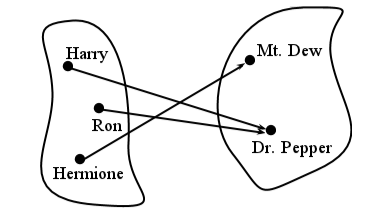
\includegraphics[width=0.9\textwidth]{function.png}
\caption{A function represented graphically.}
\label{function}
\end{figure}

This simply shows which elements of the domain map to which elements of the
codomain. The left blob is the domain, the right blob is the codomain, and
there's an arrow representing each mapping.

Now as with relations, functions normally have ``meaning." We could define
a function called ``firstTasted" that associates each wizard with the soft
drink he or she \textit{first} sampled as a child. We could define another
called ``faveDrink" that maps each wizard to his or her favorite ---
presuming that every wizard has a favorite drink in the set (Hermione will
have to overlook her iced tea and choose among the options provided).  A
third function called ``wouldChooseWithMexicanFood" provides information
about which drink each wizard provides with that type of cuisine. Here are
Ron's values for each of the three functions:

\begin{center}
firstTasted(Ron) = Mt.~Dew \\
faveDrink(Ron) = Mt.~Dew \\
wouldChooseWithMexicanFood(Ron) = Dr.~Pepper
\end{center}

These values indicate that Mt.~Dew was the soda pop that Ron first sipped,
and it has been his favorite ever since, although at \textit{La Estrellita}
he prefers a Pepper.

\index{intensional}
\index{extensional}
Functions can be defined intensionally or extensionally, just as with
relations. Intensionally, we provide the conceptual meaning of what the
function represents. Extensionally, we list the values for each element of
the domain.

\index{range (of a function)}
One other term that applies to every function is its \textbf{range}. A
function's range is the subset of the codomain that at least one element
the domain actually maps to. It's the part of the codomain that's
``reachable." For instance, if the function $G : X \rightarrow Y$ is \{
(Harry, Dr.~Pepper), (Ron, Dr.~Pepper), (Hermione, Dr.~Pepper)~\}, then
even though the codomain is \{~Dr.~Pepper, Mt.~Dew~\} the \textit{range} is
merely \{~Dr.~Pepper~\}.  That's because there isn't any ordered pair that
contains Mt.~Dew, so it's left out of the range. You can't ``reach" Mt.~Dew
via the $G$ function by starting with any of its inputs, so it's left out
in the cold.

\index{image (of a function)}
By the way, a function's range is sometimes called its \textbf{image}.
These terms are synonymous.


\section{Properties of functions}

As with relations, there are certain simple properties that some (not all)
functions have, and it's useful to reason about them. A function can be:

\begin{itemize}

\index{injective (function)}
\item \textbf{Injective}. An injective function is not only a function, but
also kind of a ``function in reverse": \textit{i.e.}, not only does no $x$
map to two different $y$'s (which is the case for all functions), but no
two $x$'s map to the same $y$. In graphical terms, it \textit{does} pass a
``horizontal line test" in addition to the vertical. Note that this can't
happen if the domain is larger than the codomain (as with wizards \& soft
drinks), since there aren't enough $y$ values to accommodate all the $x$
values uniquely. So there is no injective function between wizards and soft
drinks to be found, no matter how hard we try.

The function phoneExtension --- with employees as the domain and four-digit
numbers as the codomain --- is an example of an injective function. One
mapping of this function would be ``phoneExtension(Sally) = 1317",
indicating that Sally can be reached at x1317. Some of the available
extensions may be currently unused, but every employee does have one (and
only one) which makes it a function. But since no two employees have the
\textit{same} extension, it is also an injective function.

\index{one-to-one (function)}
Injective functions are sometimes called \textbf{one-to-one} functions.
(One-to-one and injective are exact synonyms.)

\index{surjective (function)}
\item \textbf{Surjective}. A surjective function is one that reaches all
the elements of its codomain: some $x$ does in fact reach every $y$.
Another way of saying this is: for a surjective function, the range equals
the entire codomain. You can see that this is impossible if the domain is
smaller than the codomain, since there wouldn't be enough $x$ values to
reach all the $y$ values. If we added Pepsi and Barq's Root Beer to our $Y$
set, we would thereby eliminate the possibility of any surjective functions
from $X$ to $Y$ (unless we also added wizards, of course).

The function worksIn --- with employees as the domain and departments as
the codomain --- is an example of an surjective function. One mapping of
this function would be ``worksIn(Sid) = Marketing", indicating that
Sid works in the Marketing department. Each employee works for one
department, which makes it a function. But at least \textit{one} employee
works in \textit{every} department (\textit{i.e.}, there are no empty
departments with no people in them) which makes it surjective.

\index{onto (function)}
Surjective functions are sometimes called ``\textbf{onto}" functions.
(Onto and surjective are exact synonyms.)

\index{bijective (function)}
\item \textbf{Bijective}. Finally, a bijective function is simply one that
is both injective and surjective. With an injective function, every $y$ is
mapped to by \textit{at most} one $x$; with a surjective function, every
$y$ is mapped to by \textit{at least} one $x$; so with a bijective
function, every $y$ is mapped to by \textit{exactly} one $x$. Needless to
say, the domain and the codomain must have the same cardinality for this to
be possible.

The function employeeNumber --- with employees as the domain and employee
numbers as the codomain --- is a bijective function. Every employee has an
employee number, and every employee number goes with exactly one employee.
As a corollary of this, there are the same number of employees as employee
numbers.

\end{itemize}

Finally, a few extensionally-defined examples. With $X$ = \{~Harry, Ron,
Hermione~\} and $Y$ = \{~Dr.~Pepper, Mt.~Dew~\}, consider the function
$f_1$:

\begin{center}
$f_1$(Harry) = Mt.~Dew \\
$f_1$(Ron) = Mt.~Dew \\
$f_1$(Hermione) = Mt.~Dew
\end{center}

Is $f_1$ injective? \textbf{No}, since more than one wizard (all of them,
in fact) map to Mt.~Dew. Is it surjective? \textbf{No}, since \textit{no}
wizard maps to Dr.~Pepper. Is it bijective? \textbf{No}, duh, since
to be bijective it must be both injective and surjective.

Now for $f_2$, change Ron to map to Dr.~Pepper instead:

\begin{center}
$f_2$(Harry) = Mt.~Dew \\
$f_2$(Ron) = Dr.~Pepper \\
$f_2$(Hermione) = Mt.~Dew
\end{center}

Is $f_2$ injective? Still \textbf{no}, since more than one wizard maps to
Mt.~Dew. (And of course \textit{no} function between these two sets can be
injective, since there aren't enough soft drinks for each wizard to have
his/her own.) But is it surjective?  \textbf{Yes}, it is now surjective, since
\textit{every} soft drink has at least one wizard mapping to it. (Still not
bijective for obvious reasons.)

Now let's add Pepsi and Barqs Root Beer to our set
of soft drinks $Y$, so that it now has four elements: \{~Dr.~Pepper,
Mt.~Dew, Pepsi, Barqs Root Beer~\}. Consider the function $f_3$:

\begin{center}
$f_3$(Harry) = Pepsi \\
$f_3$(Ron) = Pepsi \\
$f_3$(Hermione) = Mt.~Dew
\end{center}

Is $f_3$ injective? \textbf{No}, since more than one wizard maps to
Pepsi. Is it surjective? \textbf{No}, since \textit{no} wizard maps to
Dr.~Pepper or Barqs. (And of course \textit{no} function between these two
sets can be surjective, since there aren't enough wizards for each drink to
have one.) And of course not bijective.

Now for $f_4$, change Ron to map to Dr.~Pepper instead:

\begin{center}
$f_4$(Harry) = Pepsi \\
$f_4$(Ron) = Dr.~Pepper \\
$f_4$(Hermione) = Mt.~Dew
\end{center}

Still not surjective, of course, but now it \textit{is} injective, since
no drink has more than one wizard. (Still of course not bijective.)

Finally, let's add one more wizard (Neville) to the mix for two more
examples. Let $f_5$ be:

\begin{center}
$f_5$(Harry) = Barqs Root Beer \\
$f_5$(Ron) = Dr.~Pepper \\
$f_5$(Hermione) = Mt.~Dew \\
$f_5$(Neville) = Dr.~Pepper
\end{center}

Is $f_5$ injective? \textbf{No}, since Dr.~Pepper has two wizards. Is it
surjective? \textbf{No}, since Pepsi has none. Struck out on all counts.
However, one small change and everything falls into place:

\begin{center}
$f_6$(Harry) = Barqs Root Beer \\
$f_6$(Ron) = Pepsi \\
$f_6$(Hermione) = Mt.~Dew \\
$f_6$(Neville) = Dr.~Pepper
\end{center}

Is this last function injective, surjective, bijective? \textbf{Yes} to all
three! Every wizard gets his/her own soft drink, every soft drink gets its
own wizard, and no soft drinks (or wizards) are left out. How exciting.
This is a perfectly bijective function, also called a \textbf{bijection}.
Again, the only way to get a bijection is for the domain and codomain to be
the same size (although that alone does not \textit{guarantee} a bijection;
witness $f_5$, above). Also observe that if they \textit{are} the same
size, then injectivity and surjectivity go hand-in-hand. Violate one, and
you're bound to violate the other. Uphold the one, and you're bound to
uphold the other. There's a nice, pleasing, symmetrical elegance to the
whole idea.

